\chapter{Systematischer Konzeptentwurf}
\label{cha:konzeptentwurf}
\todo[inline]{Lorem ipsum dolor sit amet, consetetur sadipscing elitr, sed diam nonumy eirmod tempor invidunt ut labore et dolore magna aliquyam erat, sed diam voluptua. At vero eos et accusam et justo duo dolores et ea rebum. Stet clita kasd gubergren, no sea takimata sanctus est Lorem ipsum dolor sit amet. Lorem ipsum dolor sit amet, consetetur sadipscing elitr, sed diam nonumy eirmod tempor invidunt ut labore et dolore magna aliquyam erat, sed diam voluptua. At vero eos et accusam et justo duo dolores et ea rebum. Stet clita kasd gubergren, no sea takimata sanctus est Lorem ipsum dolor sit amet. Lorem ipsum dolor sit amet, consetetur sadipscing elitr, sed diam nonumy eirmod tempor invidunt ut labore et dolore magna aliquyam erat, sed diam voluptua. At vero eos et accusam et justo duo dolores et ea rebum. Stet clita kasd gubergren, no sea takimata sanctus est Lorem ipsum dolor sit amet. Duis autem vel eum iriure dolor in hendrerit in vulputate velit esse molestie consequat, vel illum dolore eu feugiat nulla facilisis at vero eros et accumsan et iusto odio dignissim qui blandit praesent luptatum zzril delenit augue duis dolore te feugait nulla facilisi. Lorem ipsum dolor sit amet, consectetuer}
\pagebreak  

\section{Ausgangssituation und Rahmenbedingungen}
\label{sec:ausgangssituation}
Zu Beginn des Konzeptentwurfs wurde die Aufgabenstellung präzisiert, indem der konkrete Spielaufbau, die geltenden Spielregeln sowie weitere technische und organisatorische Rahmenbedingungen eindeutig festgelegt wurden. Diese Festlegungen sind erforderlich, um ein regelkonformes und vergleichbares Spiel zwischen Robotern unterschiedlicher Teams zu ermöglichen. Die Erarbeitung der Spezifikationen erfolgte in gemeinsamer Abstimmung aller beteiligten Parteien. Im Folgenden werden diese Spezifikationen beschrieben und die vorliegende Ausgangssituation analysiert.

\paragraph{Spielplattform}
Zur Reduktion der Systemkomplexität wird als Spielplattform eine digitale Umgebung anstelle eines physischen Bretts verwendet. Das Spiel wird von beiden Robotern auf einem Tablet des Herstellers Apple (iPad) ausgeführt. Hierfür kommt die Applikation \glqq Reverse (Othello)\grqq{} \autocite{marcarelliReverseOthello2025} zum Einsatz, die für iPad und iPhone entwickelt wurde und das gemeinsame Spielen auf einem einzelnen Endgerät ermöglicht. Es werden die Standardeinstellungen der App verwendet, wobei die implementierten Spielregeln gelten, wie sie auch in Abschnitt~\ref{sec:othello} beschrieben sind.
Die Beschränkung auf eine digitale Spielumgebung vereinfacht den Systementwurf, da das Greifen, Bewegen und Rotieren physischer Spielsteine entfällt. Dadurch wird der mechatronische und algorithmische Aufwand reduziert und eine Umsetzung innerhalb des Projektzeitraums mit den verfügbaren Komponenten ermöglicht.

\paragraph{Spielaufbau}
Das Tablet wird flach und zentriert auf einem Tisch positioniert. Eine geringe Aufbauhöhe ist anzustreben, vorzugsweise ohne Schutzhülle. Es wird die standardmäßige Darstellung des Spielfelds der App in der jeweils vorgegebenen Auflösung verwendet. Da sich Tablets in ihrer physikalischen Größe unterscheiden können, muss das Robotersystem die Spielfeldabmessungen dynamisch erfassen. Eine entsprechende Kalibrierung oder Anpassung ist vor Spielbeginn durchzuführen.
Zur Definition eines einheitlichen Größenbereichs wird das Spielfeld auf eine minimale quadratische Kantenlänge von \SI{14}{\centi\metre} (entspricht einer Darstellung auf einem iPad Air mit 11~Zoll) sowie auf eine maximale Kantenlänge von \SI{19}{\centi\metre} (entspricht einer Darstellung auf einem iPad Pro mit 13~Zoll) beschränkt. Die beiden Roboter sind auf gegenüberliegenden Spielhälften anzuordnen. Um das Spielfeld ist ein Sicherheitsabstand von mindestens \SI{5.0}{\centi\metre} einzuhalten. Zur Vermeidung von Kollisionen darf der aktive Roboter während seines Spielzugs nicht in den Ruhezustandsbereich des gegnerischen Teams eindringen. Gleichzeitig darf der pausierende Roboter seinen definierten Ruhezustandsbereich nicht verlassen. Die Benutzeroberfläche der App sowie der Spielaufbau mit eingezeichneten Bereichen und Abmessungen sind in Abbildung~\ref{fig:spielaufbau} dargestellt.

\begin{figure}[hbt]
	\centering
	\begin{tikzpicture}[scale=0.8, transform shape] 
		% Bild auf Textbreite
		\node[anchor=south west, inner sep=0] (img) at (0,0)
		{\includegraphics[width=\linewidth]{images/spielaufbau}};
		
		\begin{scope}[x={(img.south east)},y={(img.north west)},xscale=1/30,yscale=1/20]
			
			\draw[<->,line width=0.75pt, color=white] (10.5,14) -- (19.5,14) node[midway,below,font=\footnotesize,text=white,transform shape=false]{\SI{14}{\centi\metre} - \SI{19}{\centi\metre}};
			\draw[<->,line width=0.75pt, color=white] (11,5.5) -- (11,14.5) node[midway,below,rotate=90,font=\footnotesize,text=white,transform shape=false]{\SI{14}{\centi\metre} - \SI{19}{\centi\metre}};
			
			\fill[pattern=north east lines, pattern color=red!70] (0,0) rectangle (7.75,20);
			\draw[red, line width=1pt] (0,0) -- (7.75,0) -- (7.75,20) -- (0,20);
			\node[transform shape=false, align=center, inner sep=6pt, fill=white, fill opacity=0.8, text opacity=1, rounded corners=6pt, font=\normalsize] at (3.75,10) {Ruhezustands-\\bereich\\Roboter 1};
			
			\fill[pattern=north east lines, pattern color=blue!70] (22.25,0) rectangle (30,20);
			\draw[blue, line width=1pt] (30,20) -- (22.25,20) -- (22.25,0) -- (30,0);
			\node[transform shape=false, align=center, inner sep=6pt, fill=white, fill opacity=0.8, text opacity=1, rounded corners=6pt, font=\normalsize] at (26.25,10) {Ruhezustands-\\bereich\\Roboter 2};
			
			\draw[green!70!black, dashed, line width=1.0pt] (8,3) rectangle (22,17);
			\node[anchor=west,font=\normalsize,text=black,transform shape=false] at (7.75,17.75) {Sicherheitszone};
			
			\draw[<->,line width=0.75pt,color=black] (8,2) -- (10.5,2)
			node[midway,below,font=\footnotesize,transform shape=false]{\SI{5}{\centi\metre}};
			\draw[line width=0.35pt] (8,2) -- ++(0,1);
			\draw[line width=0.35pt] (8,2) -- ++(0,-0.5);
			\draw[line width=0.35pt] (10.5,2) -- ++(0,3.5);
			\draw[line width=0.35pt] (10.5,2) -- ++(0,-0.5);
			
			\draw[<->,line width=0.75pt,color=black] (19.5,2) -- (22,2)
			node[midway,below,font=\footnotesize,transform shape=false]{\SI{5}{\centi\metre}};
			\draw[line width=0.35pt] (19.5,2) -- ++(0,3.5);
			\draw[line width=0.35pt] (19.5,2) -- ++(0,-0.5);
			\draw[line width=0.35pt] (22,2) -- ++(0,1);
			\draw[line width=0.35pt] (22,2) -- ++(0,-0.5);
			
%			\draw[step=1, gray!60, very thin] (0,0) grid (30,20);
%			\draw[red, line width=0.6pt] (0,0) rectangle (30,20);

		\end{scope}
	\end{tikzpicture}
	\vspace{0.5\baselineskip}
	\caption[Spielaufbau mit Sicherheits- und Ruhezonen]{Spielaufbau mit Sicherheits- und Ruhezonen.}	
	\label{fig:spielaufbau}
\end{figure}

\paragraph{Spielablauf und Zeitregelung}
Wie in den Spielregeln definiert, beginnt der Spieler Schwarz, welcher durch Zufall bestimmt wird. Anschließend werden die Spielzüge abwechselnd durchgeführt, wobei die maximale Dauer eines einzelnen Spielzugs auf \SI{2}{\minute} begrenzt ist. Diese Zeitvorgabe kann im Verlauf des Projekts im gegenseitigen Einvernehmen angepasst werden.
Zur Übergabe der Spielzüge zwischen den Robotern wird eine digitale Schachuhr \autocite{seanoconnorMultiPlayerChess2021} verwendet. Diese ist webbasiert, erfordert keine Registrierung und kann über mehrere Endgeräte synchronisiert werden. Die Schachuhr wird auf einem Smartphone geöffnet. Die Positionierung des Smartphones sowie die Skalierung der Webseite obliegen den jeweiligen Teams.
Der Wechsel zum nächsten Spieler erfolgt durch Betätigung einer Schaltfläche auf dem berührungsempfindlichen Bildschirm, wobei sich die farbliche Darstellung der Benutzeroberfläche entsprechend ändert. Die Funktionalitäten sowie die Benutzeroberfläche der Schachuhr sind in Abbildung~\ref{fig:multi-player-chess-clock} dargestellt. Die Schachuhr dient ausschließlich der Zugübergabe und nicht der Erfassung der tatsächlichen Zugspielzeit.


\begin{figure}[hbt]
	\centering
	% tikz/reversi-board.tex
% Reversi/Othello board (8x8) as reusable TikZ macros (no tikzpicture).
% Convention: A1 is top-left. Internal indices: A1 -> (0,7).

% ==========================================================
% Parameters (cell units / cell fractions)
% - Anything used in "circle(...)" is in cell units (like \rvMoveRad).
% - Line widths and node sizes need TeX lengths -> derived from cell length.
% ==========================================================
\providecommand{\rvBoardColor}{green!35}

% Geometry (CELL UNITS)
% Stones are drawn like moves: radius in cell units.
\providecommand{\rvStoneRad}{0.4}      % 0.50 => diameter exactly 1 cell
\providecommand{\rvMoveRad}{0.4}       % move marker radius (cell units)
\providecommand{\rvLastMoveRad}{0.1}   % last-move dot radius (cell units)

% Line widths (CELL FRACTIONS of one cell)
\providecommand{\rvOuterLWFrac}{0.2}
\providecommand{\rvGridLWFrac}{0.1}
\providecommand{\rvStoneLWFrac}{0.4}
\providecommand{\rvMoveLWFrac}{0.4}
\providecommand{\rvLastMoveLWFrac}{0.4}
\providecommand{\rvMarkLWFrac}{1.0}

% Flip marker (CELL UNITS + line width as fraction)
\providecommand{\rvFlipLineLWFrac}{1.0}
\providecommand{\rvFlipYmin}{0.38}
\providecommand{\rvFlipYmax}{0.62}
\providecommand{\rvFlipTriH}{0.13}
\providecommand{\rvFlipTriW}{0.12}

% Text
\providecommand{\rvCoordFont}{\small}
\providecommand{\rvValueScale}{0.95}

% ==========================================================
% Internal lengths (defined once even if file is input multiple times)
% ==========================================================
\makeatletter
\@ifundefined{rvCellLen}{\newlength{\rvCellLen}}{}
\@ifundefined{rvOuterLW}{\newlength{\rvOuterLW}}{}
\@ifundefined{rvGridLW}{\newlength{\rvGridLW}}{}
\@ifundefined{rvStoneLW}{\newlength{\rvStoneLW}}{}
\@ifundefined{rvMoveLW}{\newlength{\rvMoveLW}}{}
\@ifundefined{rvLastMoveLW}{\newlength{\rvLastMoveLW}}{}
\@ifundefined{rvMarkLW}{\newlength{\rvMarkLW}}{}
\@ifundefined{rvFlipLineLW}{\newlength{\rvFlipLineLW}}{}
\makeatother

% ==========================================================
% Scale derivation (recomputed when drawing a board)
% ==========================================================
\providecommand{\rvSetupScale}{%
	\pgfextractx{\rvCellLen}{\pgfpoint{1}{0}}%
	\pgfmathsetlength{\rvOuterLW}{\rvOuterLWFrac*\rvCellLen}%
	\pgfmathsetlength{\rvGridLW}{\rvGridLWFrac*\rvCellLen}%
	\pgfmathsetlength{\rvStoneLW}{\rvStoneLWFrac*\rvCellLen}%
	\pgfmathsetlength{\rvMoveLW}{\rvMoveLWFrac*\rvCellLen}%
	\pgfmathsetlength{\rvLastMoveLW}{\rvLastMoveLWFrac*\rvCellLen}%
	\pgfmathsetlength{\rvMarkLW}{\rvMarkLWFrac*\rvCellLen}%
	\pgfmathsetlength{\rvFlipLineLW}{\rvFlipLineLWFrac*\rvCellLen}%
}

% ==========================================================
% Board
% ==========================================================
\providecommand{\rvBoard}{%
	\rvSetupScale%
	\def\N{8}%
	\fill[\rvBoardColor] (0,0) rectangle (\N,\N);
	\draw[line width=\rvOuterLW] (0,0) rectangle (\N,\N);
	\foreach \i in {1,...,7}{%
		\draw[line width=\rvGridLW] (\i,0) -- (\i,\N);
		\draw[line width=\rvGridLW] (0,\i) -- (\N,\i);
	}%
}

\providecommand{\rvCoords}{%
	\def\N{8}%
	\foreach \x/\lab in {1/A,2/B,3/C,4/D,5/E,6/F,7/G,8/H}{%
		\node[font=\rvCoordFont] at (\x-0.5,\N+0.65) {\lab};
	}%
	\foreach \r in {1,...,8}{%
		\node[font=\rvCoordFont] at (-0.65,\N-\r+0.5) {\r};
	}%
}

% ==========================================================
% Internal primitives (indices 0..7)
% Stones are drawn in cell units (like \rvMoveRad).
% ==========================================================
\providecommand{\rvStoneWhite}[2]{%
	\rvSetupScale%
	\path[draw=black, fill=white, line width=\rvStoneLW]
	(#1+0.5,#2+0.5) circle (\rvStoneRad);
}
\providecommand{\rvStoneBlack}[2]{%
	\rvSetupScale%
	\path[draw=black, fill=black, line width=\rvStoneLW]
	(#1+0.5,#2+0.5) circle (\rvStoneRad);
}

\providecommand{\rvMoveWhite}[2]{%
	\rvSetupScale%
	\draw[dashed, draw=black, line width=\rvMoveLW]
	(#1+0.5,#2+0.5) circle (\rvMoveRad);
}
\providecommand{\rvMoveBlack}[2]{%
	\rvSetupScale%
	\draw[draw=black, line width=\rvMoveLW]
	(#1+0.5,#2+0.5) circle (\rvMoveRad);
}

\providecommand{\rvMarkFrame}[2]{%
	\rvSetupScale%
	\draw[draw=red, line width=\rvMarkLW]
	(#1,#2) rectangle ++(1,1);
}

\providecommand{\rvLastMoveDot}[2]{%
	\rvSetupScale%
	\draw[draw=yellow!70!orange, fill=yellow!80!orange, line width=\rvLastMoveLW]
	(#1+0.5,#2+0.5) circle (\rvLastMoveRad);
}

\providecommand{\rvFlipSymbol}[2]{%
	\rvSetupScale%
	\draw[draw=yellow!70!orange, line width=\rvFlipLineLW, line cap=round]
	(#1+0.5, #2+\rvFlipYmin) -- (#1+0.5, #2+\rvFlipYmax);
	\path[draw=yellow!70!orange, fill=yellow!70!orange]
	(#1+0.5, #2+\rvFlipYmax+\rvFlipTriH) --
	(#1+0.5-\rvFlipTriW, #2+\rvFlipYmax) --
	(#1+0.5+\rvFlipTriW, #2+\rvFlipYmax) -- cycle;
	\path[draw=yellow!70!orange, fill=yellow!70!orange]
	(#1+0.5, #2+\rvFlipYmin-\rvFlipTriH) --
	(#1+0.5-\rvFlipTriW, #2+\rvFlipYmin) --
	(#1+0.5+\rvFlipTriW, #2+\rvFlipYmin) -- cycle;
}

\providecommand{\rvValueLabel}[3]{%
	\node[scale=\rvValueScale] at (#1+0.5,#2+0.5) {#3};
}

% ==========================================================
% Mapping: file/rank -> internal indices
% ==========================================================
\providecommand{\rvFileToX}[1]{%
	\ifnum\pdfstrcmp{#1}{A}=0 0\else
	\ifnum\pdfstrcmp{#1}{B}=0 1\else
	\ifnum\pdfstrcmp{#1}{C}=0 2\else
	\ifnum\pdfstrcmp{#1}{D}=0 3\else
	\ifnum\pdfstrcmp{#1}{E}=0 4\else
	\ifnum\pdfstrcmp{#1}{F}=0 5\else
	\ifnum\pdfstrcmp{#1}{G}=0 6\else
	\ifnum\pdfstrcmp{#1}{H}=0 7\else
	\ifnum\pdfstrcmp{#1}{a}=0 0\else
	\ifnum\pdfstrcmp{#1}{b}=0 1\else
	\ifnum\pdfstrcmp{#1}{c}=0 2\else
	\ifnum\pdfstrcmp{#1}{d}=0 3\else
	\ifnum\pdfstrcmp{#1}{e}=0 4\else
	\ifnum\pdfstrcmp{#1}{f}=0 5\else
	\ifnum\pdfstrcmp{#1}{g}=0 6\else
	\ifnum\pdfstrcmp{#1}{h}=0 7\else
	-1%
	\fi\fi\fi\fi\fi\fi\fi\fi
	\fi\fi\fi\fi\fi\fi\fi\fi
}
\providecommand{\rvRankToY}[1]{\numexpr8-#1\relax}

% ==========================================================
% User-facing API
% ==========================================================
\providecommand{\rvStoneBlackAt}[2]{\rvStoneBlack{\rvFileToX{#1}}{\rvRankToY{#2}}}
\providecommand{\rvStoneWhiteAt}[2]{\rvStoneWhite{\rvFileToX{#1}}{\rvRankToY{#2}}}
\providecommand{\rvMoveBlackAt}[2]{\rvMoveBlack{\rvFileToX{#1}}{\rvRankToY{#2}}}
\providecommand{\rvMoveWhiteAt}[2]{\rvMoveWhite{\rvFileToX{#1}}{\rvRankToY{#2}}}
\providecommand{\rvMarkFrameAt}[2]{\rvMarkFrame{\rvFileToX{#1}}{\rvRankToY{#2}}}

\providecommand{\rvStonesBlack}[1]{\foreach \p in {#1}{\expandafter\rvStoneBlackAux\p\relax}}
\providecommand{\rvStonesWhite}[1]{\foreach \p in {#1}{\expandafter\rvStoneWhiteAux\p\relax}}
\providecommand{\rvMovesBlack}[1]{\foreach \p in {#1}{\expandafter\rvMoveBlackAux\p\relax}}
\providecommand{\rvMovesWhite}[1]{\foreach \p in {#1}{\expandafter\rvMoveWhiteAux\p\relax}}
\providecommand{\rvMarkFrames}[1]{\foreach \p in {#1}{\expandafter\rvMarkFrameAux\p\relax}}
\providecommand{\rvFlips}[1]{\foreach \p in {#1}{\expandafter\rvFlipAux\p\relax}}

\providecommand{\rvLastMove}[1]{\expandafter\rvLastMoveAux#1\relax}
\def\rvLastMoveAux#1#2\relax{%
	\rvLastMoveDot{\rvFileToX{#1}}{\rvRankToY{#2}}%
}

\providecommand{\rvValueMap}[1]{\foreach \pv in {#1}{\expandafter\rvValueMapAux\pv\relax}}
\def\rvValueMapAux#1:#2\relax{%
	\expandafter\rvValueMapCoordAux#1\relax{#2}%
}
\def\rvValueMapCoordAux#1#2\relax#3{%
	\rvValueLabel{\rvFileToX{#1}}{\rvRankToY{#2}}{#3}%
}

% Coordinate parser for tokens like "E4"
\def\rvStoneBlackAux#1#2\relax{\rvStoneBlackAt{#1}{#2}}
\def\rvStoneWhiteAux#1#2\relax{\rvStoneWhiteAt{#1}{#2}}
\def\rvMoveBlackAux#1#2\relax{\rvMoveBlackAt{#1}{#2}}
\def\rvMoveWhiteAux#1#2\relax{\rvMoveWhiteAt{#1}{#2}}
\def\rvMarkFrameAux#1#2\relax{\rvMarkFrameAt{#1}{#2}}
\def\rvFlipAux#1#2\relax{\rvFlipSymbol{\rvFileToX{#1}}{\rvRankToY{#2}}}

% Matrix input to display values on board
\providecommand{\rvValueMatrix}[8]{%
	\rvValueMatrixRow{#1}{7}%
	\rvValueMatrixRow{#2}{6}%
	\rvValueMatrixRow{#3}{5}%
	\rvValueMatrixRow{#4}{4}%
	\rvValueMatrixRow{#5}{3}%
	\rvValueMatrixRow{#6}{2}%
	\rvValueMatrixRow{#7}{1}%
	\rvValueMatrixRow{#8}{0}%
}

\def\rvValueMatrixRow#1#2{%
	\foreach \v [count=\x from 0] in {#1}{%
		\rvValueLabel{\x}{#2}{\v}%
	}%
}

	\subfigure[Spieler 1 am Zug]{
	\includegraphics[width=0.2\linewidth]{images/multi-player-chess-clock-1}
	}
	\hspace{0.2\linewidth}
	\subfigure[Spieler 2 am Zug]{
	\includegraphics[width=0.2\linewidth]{images/multi-player-chess-clock-2}
	}
	\caption[Digitale Schachuhr zur Zugübergabe]{Benutzeroberfläche der digitalen Schachuhr zur Zugübergabe. In (a) ist Spieler~1 am Zug, in (b) Spieler~2. Der Spielerwechsel erfolgt durch Betätigung der hervorgehobenen Schaltfläche.}
	\label{fig:multi-player-chess-clock}
\end{figure}

\paragraph{Hardwareeinschränkungen}
Die Interaktion des Roboters mit dem Tablet erfolgt ausschließlich über einen Touchstift oder einen vergleichbaren mechanischen Betätigungsmechanismus. Die konkrete technische Ausführung, etwa in Bezug auf Geometrie, Befestigung und Art der Betätigung, ist nicht standardisiert und den jeweiligen Teams überlassen.
Für den Aufbau des Roboters dürfen ausschließlich Bauteile aus dem LEGO\textsuperscript{\textregistered} SPIKE Prime-Baukastensystem verwendet werden. Ergänzend ist der Einsatz weniger selbst gefertigter 3D-gedruckter Komponenten zulässig, beispielsweise zur Fixierung des Touchstifts. Stationäre Roboterelemente dürfen im Ruhezustandsbereich auf der Tischfläche befestigt werden, etwa mittels Klettband, Klebeband oder vergleichbarer Hilfsmittel.
Das Steuerungsprogramm des Roboters sowie der Spielalgorithmus sind vollständig auf dem im Set enthaltenen Mikrocontroller zu implementieren. Der Systemaufbau des Baukastensystems, die verfügbaren Komponenten und die Programmierumgebung werden in Abschnitt~\ref{sec:lego-spike} beschrieben.
Zu berücksichtigen ist, dass die begrenzte Anzahl an Sensoren und Aktoren sowie die eingeschränkte Rechenleistung des Mikrocontrollers wesentliche Randbedingungen für den Konzeptentwurf darstellen. Zusätzlich führen die ausschließlich steckbaren Klemmbausteinverbindungen, die Materialelastizität der Kunststoffbauteile sowie das mechanische Spiel in Getriebekomponenten und Motoren zu einer reduzierten Positioniergenauigkeit. Diese Einschränkungen sind im mechanischen und algorithmischen Entwurf entsprechend zu berücksichtigen.

\paragraph{Organisatorischer Rahmen und Projektstruktur}
Die Bearbeitung der Aufgabenstellung erfolgt in zwei zeitlich getrennten dreimonatigen Akademiephasen, deren Ergebnisse jeweils in einer Studienarbeit dokumentiert werden. Die vorliegende Arbeit widmet sich dem systematischen Konzeptentwurf sowie den algorithmischen und spieltheoretischen Grundlagen. Die praktische Umsetzung erfolgt in der anschließenden Studienarbeit. Dort werden zudem ein Turnier (\emph{Machine vs. Machine}), die Prämierung des Gewinners sowie die Präsentation des entwickelten Roboters durchgeführt.

\section{Definition und Analyse der Anforderungen}
\label{sec:anforderungen}

Basierend auf der Spezifikation der Rahmenbedingungen sowie der Analyse der Ausgangssituation werden im Folgenden die Anforderungen an das technische System definiert und analysiert. 
Das betrachtete technische System ist ein autonom agierender Roboter, dessen Aufgabe es ist, gegen einen weiteren Roboter das Spiel Othello gemäß den festgelegten Regeln, dem definierten Spielaufbau und dem vorgegebenen Ablauf auszuführen und dabei das Ziel des Gewinns zu verfolgen. Die Definition der Anforderungen dient sowohl der weiteren Konkretisierung der Aufgabenstellung als auch der Verifikation und Bewertung des erarbeiteten Konzepts.

Die nachfolgenden Anforderungen beziehen sich auf das Gesamtsystem. Hardware- und Softwarekomponenten werden dabei gemeinsam betrachtet. Eine weitergehende Zerlegung der Anforderungen auf Subsystem-, Funktions- oder Komponentenebene ist nicht Gegenstand dieser Arbeit. Gemäß \autocite{pohlBasiswissenRequirementsEngineering2021a} werden die Anforderungen in drei Kategorien unterteilt:

\begin{enumerate}
	\item \textbf{Funktionale Anforderungen (FA):}  
	Beschreiben die vom technischen System bereitzustellenden Funktionen und Verhaltensweisen. Sie legen fest, welche Aufgaben das System ausführen muss, um die Zielsetzung der Aufgabenstellung zu erfüllen.
	
	\item \textbf{Nicht-funktionale Anforderungen (NFA):}  
	Beschreiben qualitative Eigenschaften, Leistungsmerkmale oder Gütekriterien des Systems, wie beispielsweise Genauigkeit, Robustheit, Zeitverhalten oder Zuverlässigkeit. Sie konkretisieren, in welcher Qualität die funktionalen Anforderungen zu erfüllen sind.
	
	\item \textbf{Randbedingungen (RB):}  
	Definieren Einschränkungen des Lösungsraums, die sich aus organisatorischen, technischen oder projektspezifischen Vorgaben ergeben. Randbedingungen beschreiben, unter welchen Voraussetzungen und mit welchen Mitteln das System realisiert werden darf bzw. was ausdrücklich ausgeschlossen ist.
\end{enumerate}

Darüber hinaus werden die Anforderungen nach ihrer Kritikalität (Krit.) auf einer Skala von 1 bis 10 priorisiert, welche die Bedeutung einzelner Anforderungen für die Zielerreichung angibt. Die Anforderungen sind nicht als abgeschlossen zu verstehen, sondern können im Projektverlauf weiter konkretisiert, ergänzt oder angepasst werden. Eine strukturierte Übersicht der funktionalen Anforderungen, der nicht-funktionalen Anforderungen sowie der Randbedingungen ist in den Tabellen~\ref{tab:funktionale_anforderungen}, \ref{tab:nichtfunktionale_anforderungen} und \ref{tab:randbedingungen} dargestellt.

% ------------------------------------------------------------
% FUNKTIONALE ANFORDERUNGEN
% ------------------------------------------------------------
{
	\renewcommand{\arraystretch}{1.5}
	
	\begin{longtable}{
			>{\centering\arraybackslash}p{0.10\linewidth}
			p{0.72\linewidth}
			>{\centering\arraybackslash}p{0.10\linewidth}
		}
		\captionabove[Auflistung der funktionalen Anforderungen]{Auflistung der funktionalen Anforderungen an das technische System.}
		\label{tab:funktionale_anforderungen} \\
		
		\hline
		\textbf{ID} & \textbf{Funktionale Anforderung}: Das tech. System \textbf{muss} \dots & \textbf{Krit.} \\
		\hline
		\endfirsthead
		
		\hline
		\textbf{ID} & \textbf{Funktionale Anforderung}: Das tech. System \textbf{muss} \dots & \textbf{Krit.} \\
		\hline
		\endhead
		
		\hline
		\multicolumn{3}{r}{\emph{Fortsetzung auf der nächsten Seite}} \\
		\endfoot
		
		\hline
		\endlastfoot
		
		FA-1 & das Spiel Othello vollständig und regelkonform gemäß den festgelegten Spielregeln ausführen. & 10 \\
		
		FA-2 & den aktuellen Spielzustand erfassen, einschließlich der vollständigen Belegung des Spielfelds sowie der zuletzt ausgeführten gegnerischen Spielzüge. & 10 \\
		
		FA-3 & auf Basis des erfassten Spielzustands einen zulässigen und unter den gegebenen Hardwareeinschränkungen bestmöglichen Spielzug bestimmen, ohne externe Eingriffe oder Unterstützung. & 10 \\
		
		FA-4 & Spielzüge präzise und reproduzierbar über eine mechanische Touch-Eingabe auf dem Tablet ausführen und den Abschluss des Spielzugs eindeutig an den nächsten Spieler übergeben. & 9 \\
		
		FA-5 & die definierten Sicherheits- und Ruhezustandsbereiche während des gesamten Spielbetriebs jederzeit einhalten. & 10 \\
		
		FA-6 & jeden Spielzug innerhalb der maximal zulässigen Zugzeit vollständig abschließen. & 8 \\
		
	\end{longtable}
}

% ------------------------------------------------------------
% NICHT-FUNKTIONALE ANFORDERUNGEN
% ------------------------------------------------------------
{
	\renewcommand{\arraystretch}{1.5}
	
	\begin{longtable}{
			>{\centering\arraybackslash}p{0.10\linewidth}
			p{0.72\linewidth}
			>{\centering\arraybackslash}p{0.10\linewidth}
		}
		\captionabove[Auflistung der nicht-funktionalen Anforderungen]{Auflistung der nicht-funktionalen Anforderungen an das technische System.}
		\label{tab:nichtfunktionale_anforderungen} \\
		
		\hline
		\textbf{ID} & \textbf{Nicht-funktionale Anforderung}: Das techn. System \textbf{soll} \dots & \textbf{Krit.} \\
		\hline
		\endfirsthead
		
		\hline
		\textbf{ID} & \textbf{Nicht-funktionale Anforderung}: Das techn. System \textbf{soll} \dots & \textbf{Krit.} \\
		\hline
		\endhead
		
		\hline
		\multicolumn{3}{r}{\emph{Fortsetzung auf der nächsten Seite}} \\
		\endfoot
		
		\hline
		\endlastfoot
		
		NFA-1 & Touch-Eingaben auch bei geringen Lage- oder Positionierungsabweichungen des Tablets zuverlässig ausführen. & 6 \\
		
		NFA-2 & nach dem Einschalten selbstständig einen definierten und reproduzierbaren Initialzustand einnehmen. & 6 \\
		
		NFA-3 & fehlerhafte oder nicht eindeutig erkannte Touch-Eingaben erkennen und selbstständig korrigieren oder wiederholen. & 5 \\
		
		NFA-4 & Kalibrier- und Bewegungsparameter ohne Änderung des Quellcodes anpassbar halten. & 5 \\
		
	\end{longtable}
}

% ------------------------------------------------------------
% RANDBEDINGUNGEN
% ------------------------------------------------------------
{
	\renewcommand{\arraystretch}{1.5}
	
	\begin{longtable}{
			>{\centering\arraybackslash}p{0.10\linewidth}
			p{0.72\linewidth}
			>{\centering\arraybackslash}p{0.10\linewidth}
		}
		\captionabove[Auflistung der Randbedingungen]{Auflistung der Randbedingungen an das technische System.}
		\label{tab:randbedingungen} \\
		
		\hline
		\textbf{ID} & \textbf{Randbedingung}: Das techn. System \textbf{darf} bzw. \textbf{muss} \dots & \textbf{Krit.} \\
		\hline
		\endfirsthead
		
		\hline
		\textbf{ID} & \textbf{Randbedingung}: Das techn. System \textbf{darf} bzw. \textbf{muss} \dots & \textbf{Krit.} \\
		\hline
		\endhead
		
		\hline
		\multicolumn{3}{r}{\emph{Fortsetzung auf der nächsten Seite}} \\
		\endfoot
		
		\hline
		\endlastfoot
		
		RB-1 & ausschließlich Komponenten des LEGO SPIKE Prime-Baukastensystems sowie ergänzend einzelne selbst gefertigte 3D-Druckteile verwenden. & 9 \\
		
		RB-2 & Steuerungssoftware und Spielalgorithmus vollständig lokal auf dem im Baukastensystem enthaltenen Mikrocontroller ausführen und keine externe Rechner, Cloud-Dienste oder Netzwerke zur Spielentscheidung oder Zustandsbewertung verwenden.  & 8 \\
		
		RB-3 & Die Konzeption, Implementierung und Validierung des technischen Systems müssen vollständig innerhalb des vorgesehenen Projektzeitraums erfolgen. & 8 \\
		
		
	\end{longtable}
}


\section{Funktionale Analyse des Systems}
\label{sec:funktionsanalyse}
Auf Basis der definierten Anforderungen wird die Hauptfunktion des Systems in einzelne Teilfunktionen zerlegt und analysiert. Die Hauptfunktion besteht darin, gegen einen weiteren Roboter das Spiel Othello gemäß den festgelegten Regeln, dem definierten Spielaufbau und dem vorgegebenen Ablauf auszuführen und dabei das Ziel des Gewinns zu verfolgen. Die funktionale Zerlegung dient der systematischen Strukturierung des Gesamtsystems, um die Komplexität zu reduzieren und klar abgegrenzte Schnittstellen zu definieren. Dadurch können die einzelnen Teilfunktionen weitgehend unabhängig voneinander untersucht und jeweils geeignete Lösungsansätze abgeleitet werden. Die Abbildung~\ref{fig:funktionsanalyse} zeigt den anfänglichen Spielablauf sowie die Unterteilung des eigenen Spielzugs in mehrere Teilfunktionen.

- Funktion bereits vor Begin des Spielsaufbaus: Kalibierung, EInmessung des Spielfelds da größe dynamisch gestaltet wird, manueell. Es soll dabei  

\begin{figure}[hbt]
	\centering
	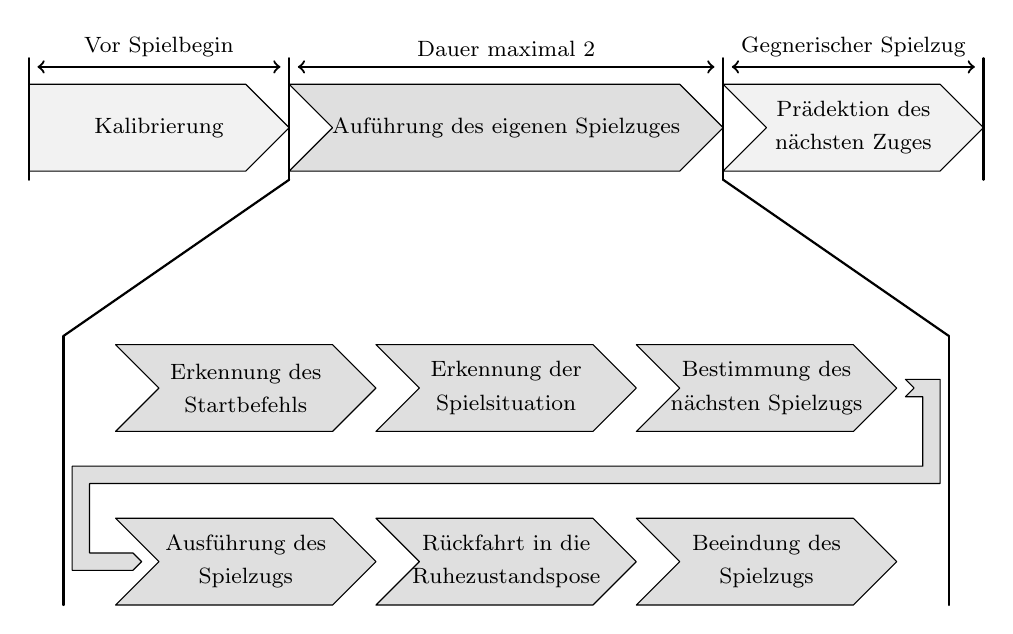
\begin{tikzpicture}[
		x=\linewidth/110, 
		y=\linewidth/110,
		line cap=round,
		line join=round
		]
		
		% -------- Parameter --------
		\def\XMAX{110}
		\def\YMAX{70}
		\def\MAJOR{10}
		\def\MINOR{1}
		
		% -------- Raster --------
		%\draw[very thin, gray!20] (0,0) grid[step=\MINOR] (\XMAX,\YMAX);
		%\draw[thin, gray!45] (0,0) grid[step=\MAJOR] (\XMAX,\YMAX);
	
		\path[draw=black, thin, fill=gray!25] (10,20) -- ++(25,0) -- ++(5,5) -- ++(-5,5) -- ++(-25,0) -- ++(5,-5) -- cycle;
		\node[align=center] at (25,25) {\footnotesize Erkennung des \\ \footnotesize Startbefehls};
		
		\path[draw=black, thin, fill=gray!25] (40,20) -- ++(25,0) -- ++(5,5) -- ++(-5,5) -- ++(-25,0) -- ++(5,-5) -- cycle;
		\node[align=center] at (55,25) {\footnotesize Erkennung der \\ \footnotesize Spielsituation};
		
		\path[draw=black, thin, fill=gray!25] (70,20) -- ++(25,0) -- ++(5,5) -- ++(-5,5) -- ++(-25,0) -- ++(5,-5) -- cycle;
		\node[align=center] at (85,25) {\footnotesize Bestimmung des \\ \footnotesize nächsten Spielzugs};
		
		\path[draw=black, thin, fill=gray!25] (10,0) -- ++(25,0) -- ++(5,5) -- ++(-5,5) -- ++(-25,0) -- ++(5,-5) -- cycle;
		\node[align=center] at (25,5) {\footnotesize Ausführung des \\ \footnotesize Spielzugs};
		
		\path[draw=black, thin, fill=gray!25] (40,0) -- ++(25,0) -- ++(5,5) -- ++(-5,5) -- ++(-25,0) -- ++(5,-5) -- cycle;
		\node[align=center] at (55,5) {\footnotesize Rückfahrt in die \\ \footnotesize Ruhezustandspose};
		
		\path[draw=black, thin, fill=gray!25] (70,0) -- ++(25,0) -- ++(5,5) -- ++(-5,5) -- ++(-25,0) -- ++(5,-5) -- cycle;
		\node[align=center] at (85,5) {\footnotesize Beeindung des \\ \footnotesize Spielzugs};
		
		\path[draw=black, thin, fill=gray!10] (0,50) -- ++(25,0) -- ++(5,5) -- ++(-5,5) -- ++(-25,0) -- cycle;
		\node[align=center] at (15,55) {\footnotesize Kalibrierung};
		
		\path[draw=black, thin, fill=gray!25] (30,50) -- ++(45,0) -- ++(5,5) -- ++(-5,5) -- ++(-45,0) -- ++(5,-5) -- cycle;
		\node[align=center] at (55,55) {\footnotesize Auführung des eigenen Spielzuges};
		
		\path[draw=black, thin, fill=gray!10] (80,50) -- ++(25,0) -- ++(5,5) -- ++(-5,5) -- ++(-25,0) -- ++(5,-5) -- cycle;
		\node[align=center] at (95,55) {\footnotesize Prädektion des\\ \footnotesize nächsten Zuges};
		
		\path[draw=black, thin, fill=gray!25] (101,26) -- ++(4,0) -- ++(0,-12) -- ++(-98,0) -- ++(0,-8) -- ++(5,0) -- ++(1,-1) -- ++(-1,-1) -- ++(-7,0) -- ++(0,12) -- ++(98,0) -- ++(0,8) -- ++(-2,0) -- ++(1,1) -- cycle;
		
		
		\draw [thick] (4, 31) -- (30, 49);
		\draw [thick] (106, 31) -- (80, 49);
		
		\draw [thick] (4, 0) -- ++(0, 31);
		\draw [thick] (106, 0) -- ++(0, 31);
		
		\draw [thick] (0, 49) -- ++(0, 14);
		\draw [thick] (30, 49) -- ++(0, 14);
		\draw [thick] (80, 49) -- ++(0, 14);
		\draw [thick] (110, 49) -- ++(0, 14);
		
		\draw[<->, thick] (1,62) -- ++(28,0)
		node[midway, above] {\footnotesize Vor Spielbegin};
		
		\draw[<->, thick] (31,62) -- ++(48,0)
		node[midway, above] {\footnotesize Dauer maximal \SI{2}{\minute}};
		
		
		\draw[<->, thick] (81,62) -- ++(28,0)
		node[midway, above] {\footnotesize Gegnerischer Spielzug};
		
	\end{tikzpicture}
	\vspace{0.5\baselineskip}
	\caption[Übersicht über Spielablauf und Teilfunktionen des eigenen Spielzugs]{Übersicht über Spielablauf und Teilfunktionen des eigenen Spielzugs.}
	\label{fig:funktionsanalyse}
\end{figure}






%
%Herleitung einer Lösung (einer Methodik, eines experimentellen Aufbaus oder von unterschiedlichen Konzepten), Lösungsbewertung und bewusste Wahl des gewählten Vorgehens. An dieser Stelle ist auch auf die Zuverlässigkeit einer Methodik oder auf die Genauigkeit von Untersuchungen einzugehen. Die Überlegungen sollen dazu helfen, mit der angestrebten Lösung die gestellten Anforderungen zu erfüllen, um schließlich die Ziele der Arbeit erreichen zu können.
%
%Bei einer Gegenüberstellung von verschiedenen Lösungsansätzen kann z.~B. eine Nutzwertanalyse helfen. Dabei sind nicht nur z.~B. die Funktion, Leistungsfähigkeit, Umsetzbarkeit und Nutzbarkeit, sondern auch z.~B. wirtschaftliche Aspekte, wie Stück-, Entwicklungskosten oder Ressourcenverbrauch zu berücksichtigen. Sehr bedeutend sind auch Aspekte der Nachhaltigkeit unter Betrachtung des gesamten Lebenszyklus einer erarbeiteten Lösung.
%
%Sowohl bei der Anforderungsdefinition, als auch bei der Lösungsfindung gibt es eine große Anzahl an verschiedenen Methoden. Eine kleine Auswahl ist in der folgenden Aufzählung zu finden.
%
%\begin{itemize}
%\item Anforderungsdefinition mithilfe des Requirements Engineering  \autocite{Pohl.2021}
%\item Systems Engineering Ansatz \autocite{Schluter.2023}
%\item Agile Entwicklungsmethodiken \autocite{Cohn.2010, Martin.2020, Wirdemann.2022}
%\item Klassische Bewertungsverfahren \autocite{Breiing.1997, Zangemeister.2014}
%\end{itemize}
%
%Ziel dieses Kapitels ist, dass auf Basis von umfassend und genau formulierten Anforderungen (ggf. auch Nicht-Zielen) eine Lösungsvielfalt erarbeitet wird, welche anschließend strukturiert bewertet wird, um eine fundierte Begründung für die angestrebte Art der Umsetzung herzuleiten.